\pdftrailerid{}
\documentclass[10pt,border=1pt]{standalone}
\usepackage[T1]{fontenc}
\usepackage{mathpazo}
\usepackage{amsmath,amssymb}
\usepackage{xcolor}
\usepackage{pgfplots}
\pgfplotsset{compat=1.18}
\usetikzlibrary{shapes.geometric,positioning,arrows.meta,calc}
\definecolor{okorange}{HTML}{E69F00}
\definecolor{oksky}{HTML}{56B4E9}
\definecolor{okgreen}{HTML}{009E73}
\definecolor{okblue}{HTML}{0072B2}
\definecolor{okverm}{HTML}{D55E00}
\definecolor{okpurple}{HTML}{CC79A7}
\colorlet{accent}{okverm}
\pgfplotsset{
  safenest/.style={
    tick label style={font=\footnotesize},
    label style={font=\small},
    title style={font=\small, align=left},
    legend style={font=\footnotesize, draw=none, fill=none, cells={anchor=west}},
    grid style={black!12, line width=0.3pt},
    axis line style={black!70, line width=0.4pt},
    tick style={black!70, line width=0.4pt},
    axis lines*=left,
  },
}
\newlength{\figwidth}
\tikzset{every node/.append style={execute at begin node={\hyphenpenalty=10000\exhyphenpenalty=10000\relax}}}
\setlength{\figwidth}{13.86cm}
\begin{document}
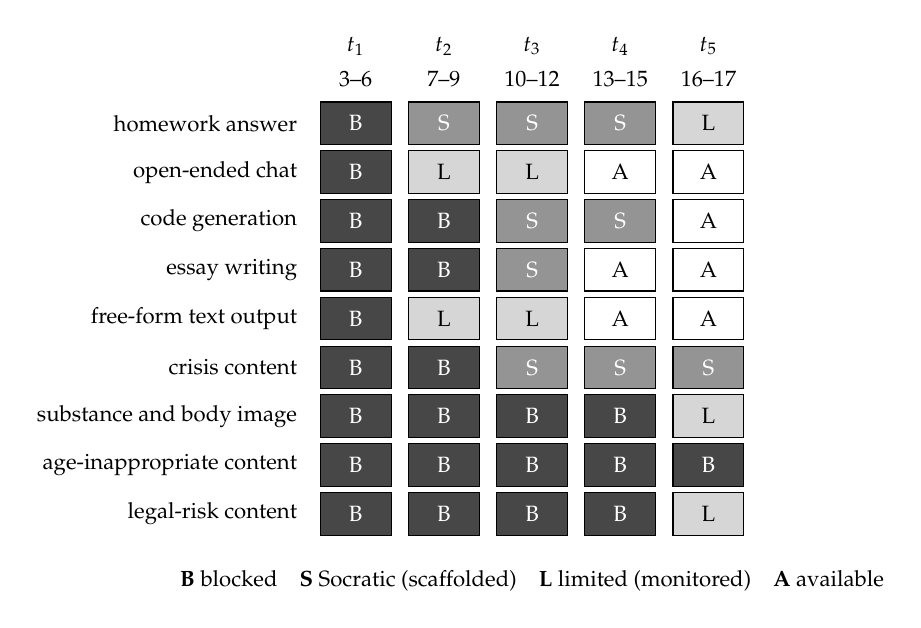
\begin{tikzpicture}[cell/.style={draw, thin, rectangle, minimum width=9mm,
                    minimum height=5.4mm, font=\footnotesize}]
\node[font=\footnotesize] at (0.00,0.98) {$t_1$};
\node[font=\footnotesize] at (0.00,0.56) {3--6};
\node[font=\footnotesize] at (1.12,0.98) {$t_2$};
\node[font=\footnotesize] at (1.12,0.56) {7--9};
\node[font=\footnotesize] at (2.24,0.98) {$t_3$};
\node[font=\footnotesize] at (2.24,0.56) {10--12};
\node[font=\footnotesize] at (3.36,0.98) {$t_4$};
\node[font=\footnotesize] at (3.36,0.56) {13--15};
\node[font=\footnotesize] at (4.48,0.98) {$t_5$};
\node[font=\footnotesize] at (4.48,0.56) {16--17};
\node[font=\footnotesize, anchor=east] at (-0.62,-0.00) {homework answer};
\node[cell, fill=black!72, text=white] at (0.00,-0.00) {B};
\node[cell, fill=black!42, text=white] at (1.12,-0.00) {S};
\node[cell, fill=black!42, text=white] at (2.24,-0.00) {S};
\node[cell, fill=black!42, text=white] at (3.36,-0.00) {S};
\node[cell, fill=black!16, text=black] at (4.48,-0.00) {L};
\node[font=\footnotesize, anchor=east] at (-0.62,-0.62) {open-ended chat};
\node[cell, fill=black!72, text=white] at (0.00,-0.62) {B};
\node[cell, fill=black!16, text=black] at (1.12,-0.62) {L};
\node[cell, fill=black!16, text=black] at (2.24,-0.62) {L};
\node[cell, fill=white, text=black] at (3.36,-0.62) {A};
\node[cell, fill=white, text=black] at (4.48,-0.62) {A};
\node[font=\footnotesize, anchor=east] at (-0.62,-1.24) {code generation};
\node[cell, fill=black!72, text=white] at (0.00,-1.24) {B};
\node[cell, fill=black!72, text=white] at (1.12,-1.24) {B};
\node[cell, fill=black!42, text=white] at (2.24,-1.24) {S};
\node[cell, fill=black!42, text=white] at (3.36,-1.24) {S};
\node[cell, fill=white, text=black] at (4.48,-1.24) {A};
\node[font=\footnotesize, anchor=east] at (-0.62,-1.86) {essay writing};
\node[cell, fill=black!72, text=white] at (0.00,-1.86) {B};
\node[cell, fill=black!72, text=white] at (1.12,-1.86) {B};
\node[cell, fill=black!42, text=white] at (2.24,-1.86) {S};
\node[cell, fill=white, text=black] at (3.36,-1.86) {A};
\node[cell, fill=white, text=black] at (4.48,-1.86) {A};
\node[font=\footnotesize, anchor=east] at (-0.62,-2.48) {free-form text output};
\node[cell, fill=black!72, text=white] at (0.00,-2.48) {B};
\node[cell, fill=black!16, text=black] at (1.12,-2.48) {L};
\node[cell, fill=black!16, text=black] at (2.24,-2.48) {L};
\node[cell, fill=white, text=black] at (3.36,-2.48) {A};
\node[cell, fill=white, text=black] at (4.48,-2.48) {A};
\node[font=\footnotesize, anchor=east] at (-0.62,-3.10) {crisis content};
\node[cell, fill=black!72, text=white] at (0.00,-3.10) {B};
\node[cell, fill=black!72, text=white] at (1.12,-3.10) {B};
\node[cell, fill=black!42, text=white] at (2.24,-3.10) {S};
\node[cell, fill=black!42, text=white] at (3.36,-3.10) {S};
\node[cell, fill=black!42, text=white] at (4.48,-3.10) {S};
\node[font=\footnotesize, anchor=east] at (-0.62,-3.72) {substance and body image};
\node[cell, fill=black!72, text=white] at (0.00,-3.72) {B};
\node[cell, fill=black!72, text=white] at (1.12,-3.72) {B};
\node[cell, fill=black!72, text=white] at (2.24,-3.72) {B};
\node[cell, fill=black!72, text=white] at (3.36,-3.72) {B};
\node[cell, fill=black!16, text=black] at (4.48,-3.72) {L};
\node[font=\footnotesize, anchor=east] at (-0.62,-4.34) {age-inappropriate content};
\node[cell, fill=black!72, text=white] at (0.00,-4.34) {B};
\node[cell, fill=black!72, text=white] at (1.12,-4.34) {B};
\node[cell, fill=black!72, text=white] at (2.24,-4.34) {B};
\node[cell, fill=black!72, text=white] at (3.36,-4.34) {B};
\node[cell, fill=black!72, text=white] at (4.48,-4.34) {B};
\node[font=\footnotesize, anchor=east] at (-0.62,-4.96) {legal-risk content};
\node[cell, fill=black!72, text=white] at (0.00,-4.96) {B};
\node[cell, fill=black!72, text=white] at (1.12,-4.96) {B};
\node[cell, fill=black!72, text=white] at (2.24,-4.96) {B};
\node[cell, fill=black!72, text=white] at (3.36,-4.96) {B};
\node[cell, fill=black!16, text=black] at (4.48,-4.96) {L};
\node[font=\footnotesize, anchor=north] at (2.24,-5.55)
  {\textbf{B} blocked\quad \textbf{S} Socratic (scaffolded)\quad
   \textbf{L} limited (monitored)\quad \textbf{A} available};
\end{tikzpicture}
\end{document}
